\chapter{Initial Data Analysis}\label{Sec:Initial Data Analysis}

In order to diagnose to what extent an algorithm suffers from sampling bias, it will be useful to have another dataset. Initial data analysis is conducted independently of the problem statements to understand what properties of the data differ between GBS and GESIS for matching attributes. A brief characterization of the data currently employed in the studies is given in this chapter. The GitHub repository further specifies the list of transformations that are sequentially applied to each group of features in order to prepare the inputs for survey comparisons. Preprocessing steps and methods used to evaluate outcomes are documented as well. Scaling methods that apply to both data sets, e.g: centering and scaling of skewed continuous features for SVMs, are not mentioned but can be deduced from code easily.

\begin{figure}[ht]
	\begin{center}
		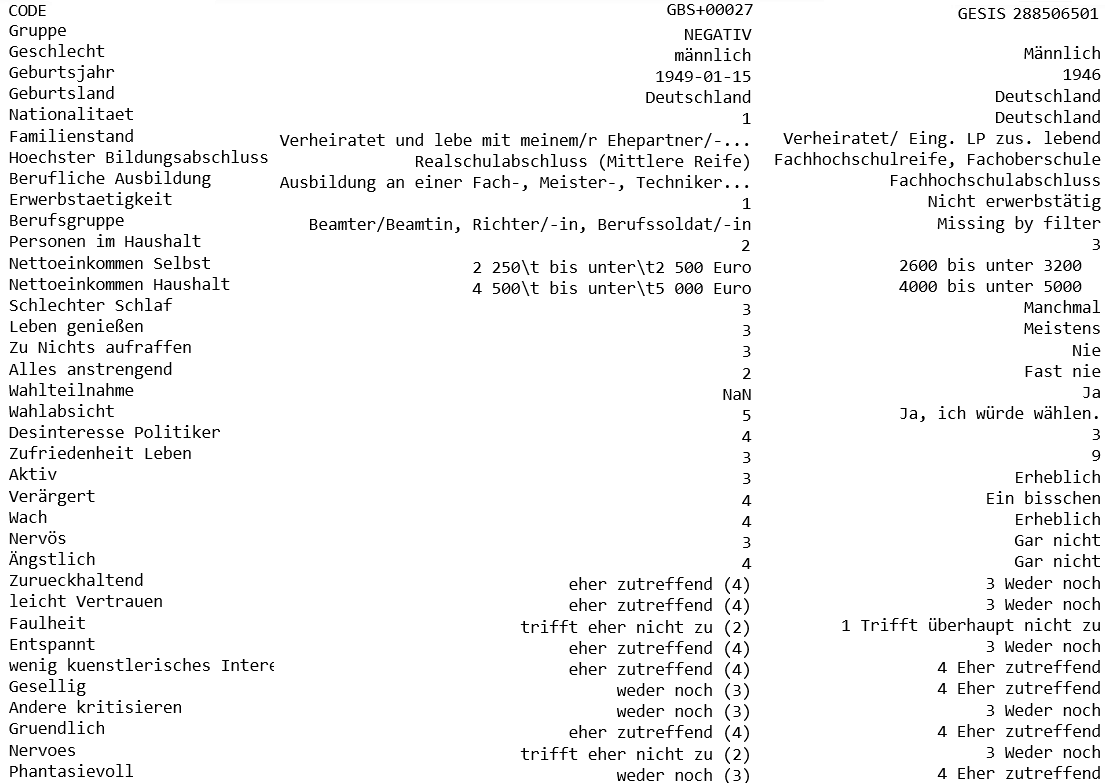
\includegraphics[scale=0.53,angle=0]{fig/values_compare}
		\label{std}
		\caption{GBS - GESIS attribute and value comparison. Not all attributes are used in every learning task. See GitHub documentation for more information.}
	\end{center}
\end{figure}

\section{Missing Data and Imputation}

\begin{figure}[ht]
	\begin{center}
		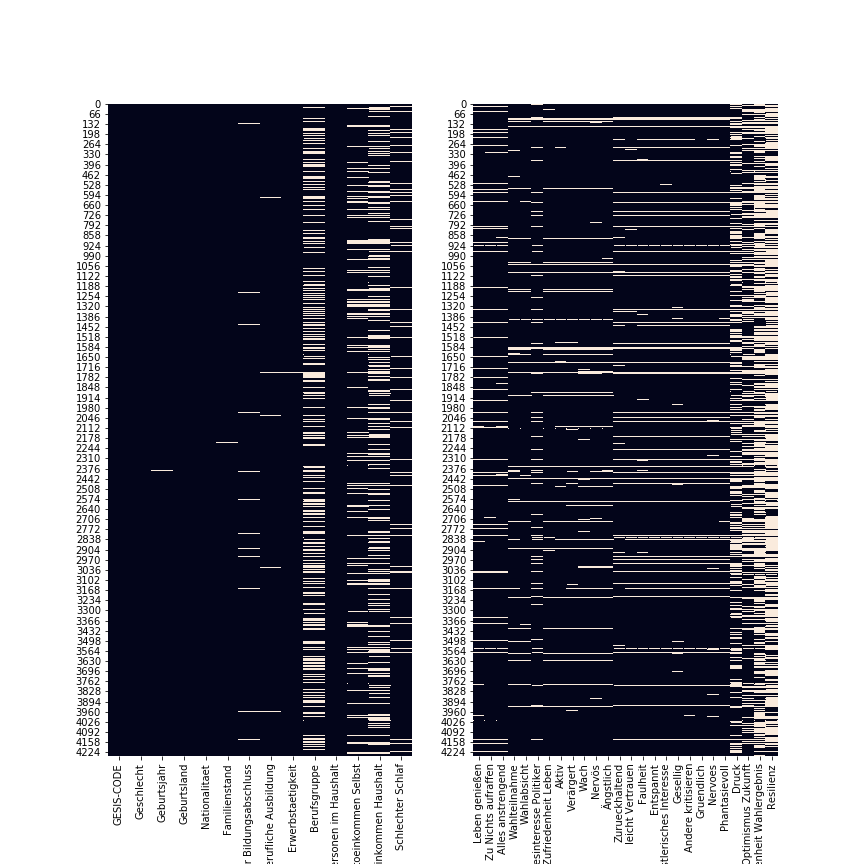
\includegraphics[scale=0.52,angle=0]{fig/gesis_missing}
		\label{std}
		\caption{GBS - GESIS attribute and value comparison.}
	\end{center}
\end{figure}

\section{Correlation Matrix}

Continuous Features First of all, we perform logarithmic transformation of the skewed continuous features in order to reduce the skewness. Second, westandardizethecontinuousfeaturesbyremovingth emeanandscalingto unit variance. Centering and scaling happen independently on each feature by computing the relevant statistics on the samples in the dataset.
Categorical Features We encode all categorical variables with values between 0 and nclasses-1 where nclasses is the number of distinct categorical values for a given variable. Next, we perform one-hot encoding.

We missing values are imputed based on domain-expert decisions. We split the input data into three groups of features: continuous, categorical and text.

\begin{figure}[ht]
	\begin{center}
		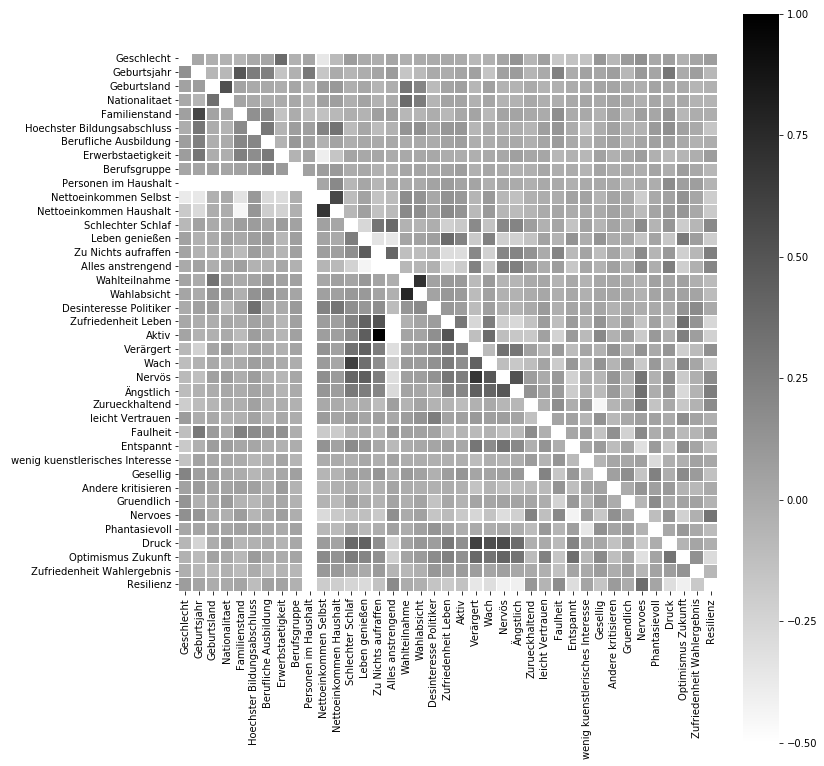
\includegraphics[scale=0.73,angle=0]{fig/correl}
		\label{std}
		\caption{GESIS missing value comparison.}
	\end{center}
\end{figure}

\section{The Big Five Dimensions}

The Big Five is an empirically-derived model of human personality and psyche. When factor analysis is applied to personality survey data, five clusters of traits consistently emerge. The BFI-10 is a 10-item scale measuring the Big Five personality traits, two BFI items for each dimension, representing both the high and low pole of each factor [Fig X]. Likert scales are the most frequently used instruments in GBS and GESIS. They consist of statements which measure the intensity of one's estimation towards the preceding statement. Respondents are asked to rate the BFI-10 items on a level of agreement on a consistent rating scale ranging from "Strongly Agree (5)" to Strongly Disagree (1)" for all items in both survey.

\begin{figure}[H]
	\begin{center}
		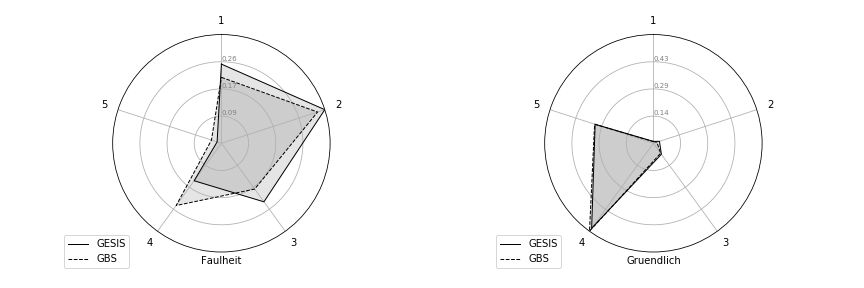
\includegraphics[scale=0.52,angle=0]{fig/Conscientiousness_figure}
		\label{Conscientiousness}
		\caption{Conscientiousness: the degree of organization, self-regulation, and responsibility one exhibits. \textit{"I see myself as someone who tends to be lazy."}(left). \textit{"I see myself as someone who does a thorough job."}(right).}
	\end{center}
\end{figure}

 is still ongoing debate on whether to use a Likert scale item as categorical or numeric feature. The intervals between positions on the scale are monotonic but never so well-defined as to be numerically uniform increments. A "Strongly Agree (5)" response indicates more agreement than "Agree", but it does not show agreement that is five times stronger than "Strongly Disagree (1)". 

There is an underlying measurement continuum, but  
This project treats the responses as if they fell on an interval scale.

Figure X. shows the response distribution of values for "Conscientiousness" of GBS and GESIS participants (see Appendix for a visualization of distribution shifts in "Agreeableness", "Openness", "Extraversion" and "Neuroticism").

Since GESIS and GBS analyse  on a group level should be relatively insensitive to problems that may arise.

In all these cases each aggregate measure (perhaps the mean) is based on many individual responses (e.g., n=50, 100, 1000, etc.). In these cases the original Likert item begins to take on properties that resemble an interval scale at the aggregate level.
life satisfaction of states or countries,
job satisfaction of departments,

The graphs are almost identical for the Likert item "Gruendlich". Kiviat diagrams are chosen over bar plots and histograms, as the data is not continuous but values are still related. The cyclic structure of the chart, i.e. "Strongly Disagree" next to Strongly Agree", provides a vivid example for the central-tendency bias across all items.

